\section{几何最优传输映射}

\subsection{Monge-Amp\'ere 方程}

\begin{problem}[Brenier] \label{pro: Brenier}
    给定$(\Omega, \mu)$和$(\sum, \nu)$以及成本函数 $c(x,y)=\frac{1}{2}\left | x-y \right |^2 $,最优传输映射$T: \Omega \to \sum$是满足Monge-Amp\'ere方程的Brenier势$u:\Omega \to \mathcal{R}$
    的梯度映射。
    \begin{equation}
        \boxed{ det \left ( \frac{\partial ^2 u(x)}{\partial x_i \partial x_j}  \right ) = \frac{f(x)}{g \circ \bigtriangledown u(x)}  }
        \label{equ:Monge-Amp\'ere}
    \end{equation}
\end{problem}

\begin{problem}[Semi-discrete OT]\label{pro: Semi-discrete OT}
    给定一个在$\mathcal{R}^d$上的紧凸域$\Omega$,和$p_1,p_2,\cdots , p_k$以及质量$w_1,w_2, \cdots , w_k >0$ ,找到一个最优传输映射$T:\Omega \to \left \{ p_1,\cdots ,p_k \right \}$,则$vol(T^{-1}(p_i))=w_i$,
    使运输成本最小化
    \begin{equation}
        C(T):=\frac{1}{2} \int _{\Omega} \left | x-T(x) \right |^2 \mathrm{d}x
        \label{equ:cost} 
    \end{equation}
\end{problem}

\begin{figure}
    [h]
	\centering
	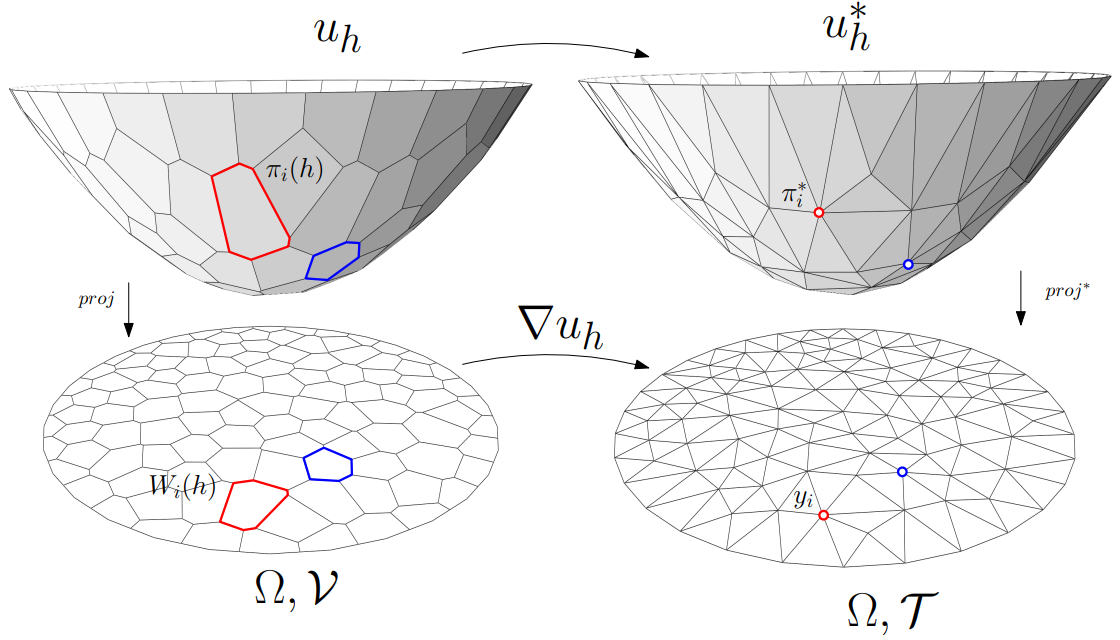
\includegraphics[width=0.6\linewidth]{Brenier}
	\caption{ Brenier图}
	\label{fig: Brenier}
\end{figure}

根据Brenier定理,将有一个分段线性凸函数$u:\Omega \to \mathbb{R}$、 梯度映射给出了最佳运输映射。

\begin{theorem}[Alexandrov 1950]
    给定在$\mathbb{R}^n$上的紧凸域$\Omega$,在$\mathbb{R}^n$上互不相同的$p_1, \cdots , p_k$,当$A_1,\cdots ,A_k >0$,使得 $\sum A_i =Vol(\Omega)$,则存在PL凸函数
    \begin{equation}
        f(x):=\max \left \{ \left \langle x,p_i \right \rangle +h_i \mid i=1, \cdots , k  \right \} ,
        \label{equ:PL convex}
    \end{equation}
    唯一的传输使得
	\begin{equation}
        Vol(W_i)=Vol\left ( \left \{ x \mid \bigtriangledown f(x)=p_i \right \}  \right ) =A_i. 
        \label{equ:Vol}
    \end{equation}
\end{theorem}

Alexandrov’s 证明是拓扑的,而不是变分。多年来人们一直开放寻找构造性的证明。

\subsection{变分证明}



\begin{algorithm}[H]
    \renewcommand{\thealgocf}{}
    \caption{\texttt{ConvexHull}($P$)}
    \KwIn{A set $P$ of points in the plane.}
    \KwOut{A list $\mathcal{L}$ containing the vertices of $\mathcal{CH}(P)$ in clockwise order.}
    Sort the points by $x$-coordinate, resulting in a sequence $p_1,...,p_n$. \\
    Put the points $p_1$ and $p_2$ in a list $\mathcal{L}_{\mathrm{upper}}$, with $p_1$ as the first point. \\
    \For {$i \leftarrow 3$ $\mathbf{to}$ $n$}
    {            
        Append $p_i$ to $\mathcal{L}_{\mathrm{upper}}$. \\
        \While {$\mathcal{L}_{\mathrm{upper}}$ contains more than $2$ points $\mathbf{and}$
                the last three points in $\mathcal{L}_{\mathrm{upper}}$ do not make a right turn}
        {
            Delete the middle of the last three points from $\mathcal{L}_{\mathrm{upper}}$.
        }
    }
    Put the points $p_n$ and $p_{n−1}$ in a list $\mathcal{L}_{\mathrm{lower}}$, with $p_n$ as the first point. \\
    \For {$i \leftarrow n - 2$ $\mathbf{down to}$ $1$}
    {            
        Append $p_i$ to $\mathcal{L}_{\mathrm{lower}}$. \\
        \While {$\mathcal{L}_{\mathrm{lower}}$ contains more than $2$ points $\mathbf{and}$
                the last three points in $\mathcal{L}_{\mathrm{lower}}$ do not make a right turn}
        {
            Delete the middle of the last three points from $\mathcal{L}_{\mathrm{lower}}$.
        }
    }
    Remove the first and the last point from $\mathcal{L}_{\mathrm{lower}}$ to avoid duplication of the points where the upper and lower hull meet. \\
    Append $\mathcal{L}_{\mathrm{lower}}$ to $\mathcal{L}_{\mathrm{upper}}$, and call the resulting list $\mathcal{L}$. \\
    \Return $\mathcal{L}$
\end{algorithm}